\documentclass[12pt,a4paper]{article}
\usepackage[polish]{babel}
\usepackage[T1]{fontenc}
\usepackage[utf8x]{inputenc}
\usepackage{hyperref}
\usepackage{url}
\usepackage[]{algorithm2e}
\usepackage{listings}

\usepackage{color}
\usepackage{listings}
\usepackage{graphicx}
\usepackage{float}

\lstloadlanguages{% Check Dokumentation for further languages ...
	C,
	C++,
	csh,
	Java
}

\definecolor{red}{rgb}{0.6,0,0} % for strings
\definecolor{blue}{rgb}{0,0,0.6}
\definecolor{green}{rgb}{0,0.8,0}
\definecolor{cyan}{rgb}{0.0,0.6,0.6}

\lstset{
	language=csh,
	basicstyle=\footnotesize\ttfamily,
	numbers=left,
	numberstyle=\tiny,
	numbersep=5pt,
	tabsize=2,
	extendedchars=true,
	breaklines=true,
	frame=b,
	stringstyle=\color{blue}\ttfamily,
	showspaces=false,
	showtabs=false,
	xleftmargin=17pt,
	framexleftmargin=17pt,
	framexrightmargin=5pt,
	framexbottommargin=4pt,
	commentstyle=\color{green},
	morecomment=[l]{//}, %use comment-line-style!
	morecomment=[s]{/*}{*/}, %for multiline comments
	showstringspaces=false,
	morekeywords={ abstract, event, new, struct,
		as, explicit, null, switch,
		base, extern, object, this,
		bool, false, operator, throw,
		break, finally, out, true,
		byte, fixed, override, try,
		case, float, params, typeof,
		catch, for, private, uint,
		char, foreach, protected, ulong,
		checked, goto, public, unchecked,
		class, if, readonly, unsafe,
		const, implicit, ref, ushort,
		continue, in, return, using,
		decimal, int, sbyte, virtual,
		default, interface, sealed, volatile,
		delegate, internal, short, void,
		do, is, sizeof, while,
		double, lock, stackalloc,
		else, long, static,
		enum, namespace, string},
	keywordstyle=\color{cyan},
	identifierstyle=\color{red},
}
\usepackage{caption}
\DeclareCaptionFont{white}{\color{white}}
\DeclareCaptionFormat{listing}{\colorbox{blue}{\parbox{\textwidth}{\hspace{15pt}#1#2#3}}}
\captionsetup[lstlisting]{format=listing,labelfont=white,textfont=white, singlelinecheck=false, margin=0pt, font={bf,footnotesize}}


\addtolength{\hoffset}{-1.5cm}
\addtolength{\marginparwidth}{-1.5cm}
\addtolength{\textwidth}{3cm}
\addtolength{\voffset}{-1cm}
\addtolength{\textheight}{2.5cm}
\setlength{\topmargin}{0cm}
\setlength{\headheight}{0cm}

\begin{document}
	
	\title{Modelowanie i analiza systemów informatycznych \\\small{dokumentacja projektu}}
	\author{Oliwia Gowor, Hubert Kwiatkowski, Miłosz Prządka}
	\date{\today}

	\maketitle
	\newpage
	\section*{Część I}
	\subsection*{Opis programu}
	Program symuluje dynamiczną grę strategiczną opartą na planszy, w której gracze (zarówno użytkownicy, jak i agenci) rywalizują ze sobą. poprzez przemieszczanie się po planszy w celu osiągnięcia celu lub eliminacji przeciwników. Każda rozgrywka odbywa się na siatce reprezentującej planszę, a uczestnicy podejmują decyzje o ruchach na podstawie danych o otoczeniu. Gra może być używana do celów rozrywkowych, edukacyjnych (np. nauka programowania sztucznej inteligencji) lub jako platforma testowa do rozwijania i optymalizacji algorytmów AI.

	\subsection*{Instrukcja wdrożenia}
    Program można uruchomić lokalnie, korzystając z terminala. Wdrożenie jest szybkie i wymaga  spełnienia wymagań systemowych: środowiska Python w wersji 3.9 lub nowszej oraz biblioteki `curses`, która jest standardowo dostępna w systemach Linux.
   \break 

\textbf{Kroki:}
\begin{enumerate}
    \item Pobranie kodu ze źródła
    
Pierwszym krokiem jest skopiowanie projektu na lokalny komputer, np. używając `git clone` lub innej metody dystrybucji kodu.

    \item Instalacja Python 3.9+
    
Należy upewnić się, że na komputerze zainstalowana jest wersja Pythona 3.9 lub nowsza:

- W systemie Linux:

\begin{enumerate}
    \item\textbf{sudo apt update} \\
    \item \textbf{sudo apt install python3}
\end{enumerate}

- W systemie Windows:
Należy pobrać instalator Pythona i wykonać instalację.

    \item  Uruchomienie programu
    
Ostatnim krokiem jest przejście do katalogu projektu w terminalu i uruchomienie aplikacji poleceniem:

\begin{enumerate}
    \textbf{python main.py}
\end{enumerate}

    \item Dodatkowe informacje
    
- Jeśli wykorzystywany jest system Windows, konieczne może być zainstalowanie alternatywnej biblioteki obsługującej `curses`, np. `windows-curses`, za pomocą polecenia:
\end{enumerate}

\begin{enumerate}
     \textbf{pip install windows-curses}
\end{enumerate}

   - W systemach Linux i macOS `curses` jest instalowane domyślnie.
 
 \break
Program jest gotowy do użycia natychmiast po uruchomieniu. 

	\subsection{Instrukcja obsługi}
Plansza gry oraz instrukcje dotyczące sterowania są wyświetlane bezpośrednio w terminalu. Nawigacja po programie odbywa się za pomocą wpisywania odpowiednich znaków w terminalu. Gracze sterują ruchem za pomocą klawiszy (\verb|W|, \verb|S|, \verb|A|, \verb|D|), wybierając jeden z czterech kierunków (odpowiednio: góra, dół, lewo, prawo). Agenci podejmują decyzje w oparciu o algorytmy oceny sytuacji na planszy, takie jak analiza bliskości przeciwników czy unikanie kolizji. Agenci są autonomiczni i nie są im przekazywane żadne obiekty, wywoływane są tylko publiczne funkcje. Agentom losowo zostaje przypisana jedna z dostępnych taktyk gry (standardowa lub agresywna).

W grze dostępne są dwa tryby:
    \begin{itemize}
        \item \textbf{Gracz vs. Agenci:} Użytkownik wciela się w rolę jednego z graczy i rywalizuje z agentami kontrolowanymi przez algorytmy.
        \item \textbf{Agenci vs. Agenci:} Rozgrywka odbywa się wyłącznie pomiędzy agentami, a użytkownik może obserwować ich zachowanie w celach analizy i porównań.
    \end{itemize}

Gra kończy się, gdy jeden z graczy spełni warunki zwycięstwa poprzez eliminację wszystkich przeciwników.


	\newpage
	\section*{Część II}
	\subsection*{Opis działania} 
	System gry opiera się na matematycznym modelu siatki, gdzie plansza to macierz o wymiarach 20x20. Każdy gracz, będący obiektem na planszy, posiada pozycję , kierunek ruchu oraz stan (aktywny, zniszczony).
    \bigskip
	
	\textbf{Model matematyczny systemu i jego komponentów}

Model matematyczny gry jest zbudowany w oparciu o siatkę (planszę) oraz zestaw reguł opisujących interakcje między graczami i elementami planszy.

\begin{enumerate}
\item Plansza\\
Plansza jest reprezentowana jako macierz dwuwymiarowa o wymiarach , gdzie:

$M$: liczba wierszy (wysokość planszy),

$N$: liczba kolumn (szerokość planszy).\\
Każda komórka planszy  może przyjąć jedną z następujących wartości:

\begin{itemize}
    \item "..": pusta przestrzeń,
    \item $P_{k}$: pozycja gracza,
    \item $A_{k}$: pozycja agenta.
\end{itemize}

\item Pozycja gracza/agenta\\
Pozycja każdego gracza jest definiowana jako wektor współrzędnych , gdzie $x_{k}$ to kolumna, a $y_{k}$ to wiersz na planszy. Ruch gracza polega na zmianie jego pozycji zgodnie z wektorem przesunięcia $d$, tj.:

$\mathbf{p}_k^{\text{nowa}} = \mathbf{p}_k + \mathbf{d}$,
gdzie $d$:
    \begin{itemize}
        \item UP→(0,−1),
        \item DOWN→(0,+1)
        \item LEFT→(−1,0),
        \item RIGHT→(+1,0).
    \end{itemize}

\item Decyzje agentów:\\
Funkcje decyzyjne, takie jak:
\begin{itemize}
    \item Funkcja bazowa opiera się na ocenie dostępnych kierunków $D$ w postaci: \\
    $D=\{(x',y')∣x'=x+\delta x,y'=y+\deltay\cdot i\cdot M[x'][y']='..'\}$.
    \item Funkcja oceny punktowej dla kierunku $d$: $Score(d)=Reward(d)-Penalty(d)$.
\end{itemize}

\item Zasady kolizji:\\
Gracz koliduje, jeśli:
\begin{itemize}
    \item Wyjdzie poza granice planszy: $x<0∨x≥W∨y<0∨y≥H$.
    \item Wykona ruch na zajęte pole: $M[x][y]≠'..'$.
\end{itemize}
\end{enumerate}
\bigskip

\textbf{Technika rozwiązania i projektowanie systemu}\\
Program został zaprojektowany w oparciu o modularną architekturę, co ułatwia rozwój, testowanie i modyfikację komponentów. System wykorzystuje także wzorce projektowe.


\begin{enumerate}
    \item \textbf{Wzorce projektowe}:
    \begin{itemize}
        \item \textbf{Strategia}: Decyzje agentów implementowane jako różne strategie (\verb|Agent|, \verb|AggressiveAgent|).
        \item \textbf{Fabryka}: Metoda \verb|create_game| generuje graczy w zależności od trybu gry.
        \item \textbf{MVC (Model-View-Controller)}: Plansza i mechanika gry stanowią Model, interfejs terminalowy to Widok, a sterowanie graczami (w tym decyzje) to Kontroler.
    \end{itemize}
    \item \textbf{Podział na komponenty}:
    \begin{itemize}
        \item \textbf{Gracz}: Klasa bazowa, wspierająca ruch i kolizje.
        \item \textbf{Agent}: Klasa potomna z różnymi strategiami decyzyjnymi.
        \item \textbf{Watchtower}: Klasa odpowiedzialna za analizę planszy i rekomendacje ruchów.
        \item \textbf{Game}: Klasa centralna, integrująca planszę, graczy i logikę gry.
    \end{itemize}
\end{enumerate}

\subsubsection{}
\bigskip

\textbf{Techniki implementacyjne}\\
Algorytmy sterowania agentami opierają się na przeszukiwaniu lokalnym, tj. analizie możliwych ruchów i ich oceny w danej turze. Gra działa w trybie turowym, gdzie w każdej turze każdy gracz (lub agent) wykonuje jeden ruch.
\bigskip

\textbf{Zabezpieczenia i odporność na ataki}

\begin{enumerate}
    \item \textbf{Walidacja danych wejściowych}:
    \begin{itemize}
        \item Funkcje sprawdzają, czy ruch jest w granicach planszy (\verb|is_within_bounds|).
        \item Gracze są umieszczani na pustych polach przy użyciu \verb|random_empty_position|.
    \end{itemize}
    \item \textbf{Zapobieganie błędom logicznym}:
Kolizje i błędy ruchu są obsługiwane przez flagę \verb|crashed|.

    \item \textbf{Odporność na złośliwe zachowania}:
    \begin{itemize}
        \item Gra jest izolowana, bez możliwości wprowadzenia kodu zewnętrznego.
        \item Mechanizmy wykluczają ruchy poza planszę i zapobiegają konfliktom pozycji.
    \end{itemize}
\end{enumerate}

	
\subsection*{Algorytmy}
Standardowy wybór kierunku (get\textunderscore suggestion)
Metoda ta sugeruje ruch agenta, który jest oparty na analizie dostępnych kierunków w oparciu o ich ocenę. W przypadku naruszenia reguł gry, wybierany jest bezpieczny kierunek.


Ocena kierunków (\textunderscore evaluate\textunderscore directions):
\begin{itemize}
    \item Dla każdej możliwej pozycji (np. ruch "UP", "DOWN", "LEFT", "RIGHT") obliczana jest punktacja.
    \item Kierunki są oceniane według: 
        \begin{itemize}
            \item Liczby wolnych pól w otoczeniu (im więcej wolnych pól, tym lepiej).
            \item Kar za obecność innych agentów w bliskiej odległości (karana jest odległość 1 lub 2 pola).
        \end{itemize}
    \item Wynikiem jest kierunek o najwyższej punktacji. W razie braku jednoznacznego wyniku wybierany jest losowy ruch.
\end{itemize}

\begin{algorithm}[H]
\KwData{agent, game}
\KwResult{Najlepszy kierunek ruchu}

$x, y \gets$ pozycja agenta (agent.position)\;
directions $\gets \{\text{``UP'': (0, -1), ``DOWN'': (0, 1), ``LEFT'': (-1, 0), ``RIGHT'': (1, 0)}\}$\;

best\_direction $\gets \text{null}$\;
best\_score $\gets -\infty$\;

\ForEach{\textnormal{kierunek, (dx, dy)} w directions}{
    $new\_x \gets x + dx$\;
    $new\_y \gets y + dy$\;

    \If{$0 \leq new\_x < \text{game.width}$ i $0 \leq new\_y < \text{game.height}$}{
        \If{\textnormal{game.board[new\_y][new\_x] == ``..''}}{
            $score \gets \text{evaluate\_move(new\_x, new\_y, agent, game)}$\;

            \If{$score > best\_score$}{
                $best\_score \gets score$\;
                $best\_direction \gets$ kierunek\;
            }
        }
    }
}

\Return{best\_direction, jeśli istnieje, w przeciwnym razie losowy kierunek z directions}\;

\caption{Algorytm wyboru najlepszego kierunku ruchu dla agenta.}
\end{algorithm}

Sprawdzenie zgodności z zasadami (is\textunderscore within\textunderscore bounds):
Upewnia się, że ruch nie wychodzi poza granice planszy.

\begin{algorithm}[H]
\KwData{direction, x, y, game}
\KwResult{Czy nowa pozycja mieści się w granicach planszy?}

$dx, dy \gets \text{directions[direction]}$\;
$new\_x \gets x + dx$\;
$new\_y \gets y + dy$\;

\Return{$0 \leq new\_x < \text{game.width}$ oraz $0 \leq new\_y < \text{game.height}$}\;

\caption{Sprawdzenie, czy nowa pozycja mieści się w granicach planszy.}
\end{algorithm}


Bezpieczny kierunek (get\textunderscore safe\textunderscore direction):
Wybierany jest taki kierunek, który nie tylko mieści się w granicach planszy, ale także prowadzi na wolne pole.

\begin{algorithm}[H]
\KwData{directions, x, y, game}
\KwResult{Pierwszy kierunek prowadzący do wolnego pola w granicach planszy}

\ForEach{\textnormal{kierunek, (dx, dy)} w directions}{
    $new\_x \gets x + dx$\;
    $new\_y \gets y + dy$\;

    \If{$0 \leq new\_x < \text{game.width}$ oraz $0 \leq new\_y < \text{game.height}$ oraz \textnormal{game.board[new\_y][new\_x] == ``..''}}{
        \Return{kierunek}\;
    }
}
\caption{Znajdowanie pierwszego wolnego kierunku w granicach planszy.}
\end{algorithm}

Agresywny wybór kierunku (get\textunderscore aggressive\textunderscore suggestion)
Metoda ta również sugeruje ruch agenta, ale skupia się na bardziej ofensywnej strategii, nagradzając zbliżanie się do przeciwników oraz próbę ich ograniczenia.

Proces analizy
Ocena kierunków (\textunderscore evaluate\textunderscore directions\textunderscore aggressive):
Działa podobnie jak w przypadku standardowej analizy, ale ocenia ruchy na podstawie innych kryteriów:
\begin{itemize}
    \item Nagroda za bliskość do przeciwników (większa za bezpośrednią bliskość, mniejsza za odległość do 3 pól).
    \item Ocena potencjalnych ruchów, które mogą ograniczyć manewry przeciwnika (mechanizm "trap potential").
    \item Kara za wybór pól blisko krawędzi planszy (mniejsza możliwość manewrowania).
    \item Kara za zwiększanie dystansu od przeciwnika.
\end{itemize}

\begin{algorithm}[H]
\KwData{directions, x, y, game, agent}
\KwResult{Najlepszy kierunek na podstawie oceny agresywnej}

best\_direction $\gets \text{null}$\;
best\_score $\gets -\infty$\;

\ForEach{\textnormal{kierunek, (dx, dy)} w directions}{
    $new\_x \gets x + dx$\;
    $new\_y \gets y + dy$\;

    \If{$0 \leq new\_x < \text{game.width}$ oraz $0 \leq new\_y < \text{game.height}$}{
        \If{\textnormal{game.board[new\_y][new\_x] == ``..''}}{
            $score \gets \text{evaluate\_aggressive\_move(new\_x, new\_y, agent, game)}$\;

            \If{$score > best\_score$}{
                $best\_score \gets score$\;
                $best\_direction \gets$ kierunek\;
            }
        }
    }
}

\Return{best\_direction, jeśli istnieje, w przeciwnym razie losowy kierunek z directions}\;

\caption{Algorytm wyboru najlepszego kierunku ruchu z oceną agresywną.}
\end{algorithm}


Sprawdzenie zgodności z zasadami:
Analogiczne do standardowego wyboru, ale z priorytetem dla strategii agresywnej.

Ruch maksymalizujący ofensywę (get\textunderscore best\textunderscore aggressive\textunderscore move):
Szuka najlepszego ruchu na podstawie najwyższej punktacji w ocenie agresywnej.

\begin{algorithm}[H]
\KwData{directions, x, y, game, agent}
\KwResult{Najlepszy kierunek na podstawie agresywnej strategii}

best\_direction $\gets \text{null}$\;
best\_score $\gets -\infty$\;

\ForEach{\textnormal{kierunek, (dx, dy)} w directions}{
    $new\_x \gets x + dx$\;
    $new\_y \gets y + dy$\;

    \If{$0 \leq new\_x < \text{game.width}$ oraz $0 \leq new\_y < \text{game.height}$}{
        \If{\textnormal{game.board[new\_y][new\_x] == ``..''}}{
            $score \gets \text{evaluate\_aggressive\_move(new\_x, new\_y, agent, game)}$\;

            \If{$score > best\_score$}{
                $best\_score \gets score$\;
                $best\_direction \gets$ kierunek\;
            }
        }
    }
}

\Return{best\_direction, jeśli istnieje, w przeciwnym razie losowy kierunek z directions}\;

\caption{Algorytm wyboru najlepszego kierunku ruchu w oparciu o agresywną strategię.}
\end{algorithm}

	\subsection*{Implementacja systemu}
	
    \textbf{Podział na pliki}\\
System został zaprojektowany z podziałem na cztery główne moduły: \verb|agent.py|, \verb|watchtower.py|, \verb|game.py| oraz \verb|main.py|. Każdy z plików pełni odrębną funkcję w systemie, co ułatwia jego rozwój i utrzymanie.
\bigskip

\verb|agent.py|\\
Ten moduł zawiera klasy definiujące zachowanie graczy, zarówno kontrolowanych przez użytkownika, jak i przez komputer. W szczególności:
\begin{itemize}
    \item Klasa \verb|Player|:
    Reprezentuje podstawowego gracza w grze.
    Utrzymuje informacje o stanie gracza, takie jak pozycja, symbol na planszy, aktualny kierunek ruchu i status kolizji.
    Obsługuje funkcję move, która aktualizuje pozycję gracza na planszy w oparciu o obecny kierunek.
    
    \item Klasa \verb|Agent|:
    Dziedziczy po klasie Player i implementuje algorytmy decydujące o kierunku ruchu agenta.
    Funkcja decide\_move pozwala agentowi na podjęcie decyzji o ruchu, opierając się na sugestiach z Watchtower.

    \item Klasa \verb|AggressiveAgent|:
    Rozszerza klasę Agent, modyfikując jej logikę w kierunku bardziej agresywnego stylu gry.
    Agresywny agent stara się podejmować decyzje, które zwiększają presję na przeciwników, np. zbliżanie się do nich lub próby ich blokowania.
\end{itemize}
\bigskip

\verb|watchtower.py|\\
Moduł ten pełni funkcję "wieży strażniczej", która ocenia sytuację na planszy i generuje sugestie ruchu dla agentów.

    \begin{itemize}
        \item Funkcja \verb|get_suggestion| sugeruje ruch w sposób defensywny, unikając kolizji i starając się utrzymać agenta w bezpiecznej pozycji.
        \item Funkcja \verb|get_aggressive_suggestion| ocenia najlepszy możliwy ruch w sposób bardziej ofensywny, np. poprzez zbliżanie się do przeciwników.
        \item Wbudowane metody, takie jak \verb|is_within_bounds| czy \verb|get_safe_direction|, zapewniają, że ruchy są zgodne z zasadami gry i nie wychodzą poza granice planszy.
    \end{itemize}
\bigskip

\verb|game.py|\\
Ten moduł definiuje logikę gry oraz operacje na planszy.

    \begin{itemize}
        \item Klasa \verb|Game|:
Tworzy planszę gry o określonych wymiarach i inicjuje graczy na losowych, pustych pozycjach. Odpowiada za aktualizację stanu planszy w każdej turze oraz za sprawdzanie, czy gra się zakończyła. Funkcja update przesuwa graczy, sprawdza kolizje i aktualizuje ich statusy na planszy.
    \end{itemize}
\bigskip

\verb|main.py|\\
Plik \verb|main.py| pełni rolę punktu wejścia do aplikacji. Obsługuje interfejs użytkownika przy użyciu biblioteki curses. Umożliwia wybór trybu gry: "User vs Computer" lub "Computer Only". Implementuje główną pętlę gry (\verb|game_loop|), która steruje interakcjami gracza, agentami i aktualizacjami stanu gry.
\bigskip

\textbf{Diagram klas}\\
\begin{figure}[H]
    \centering
    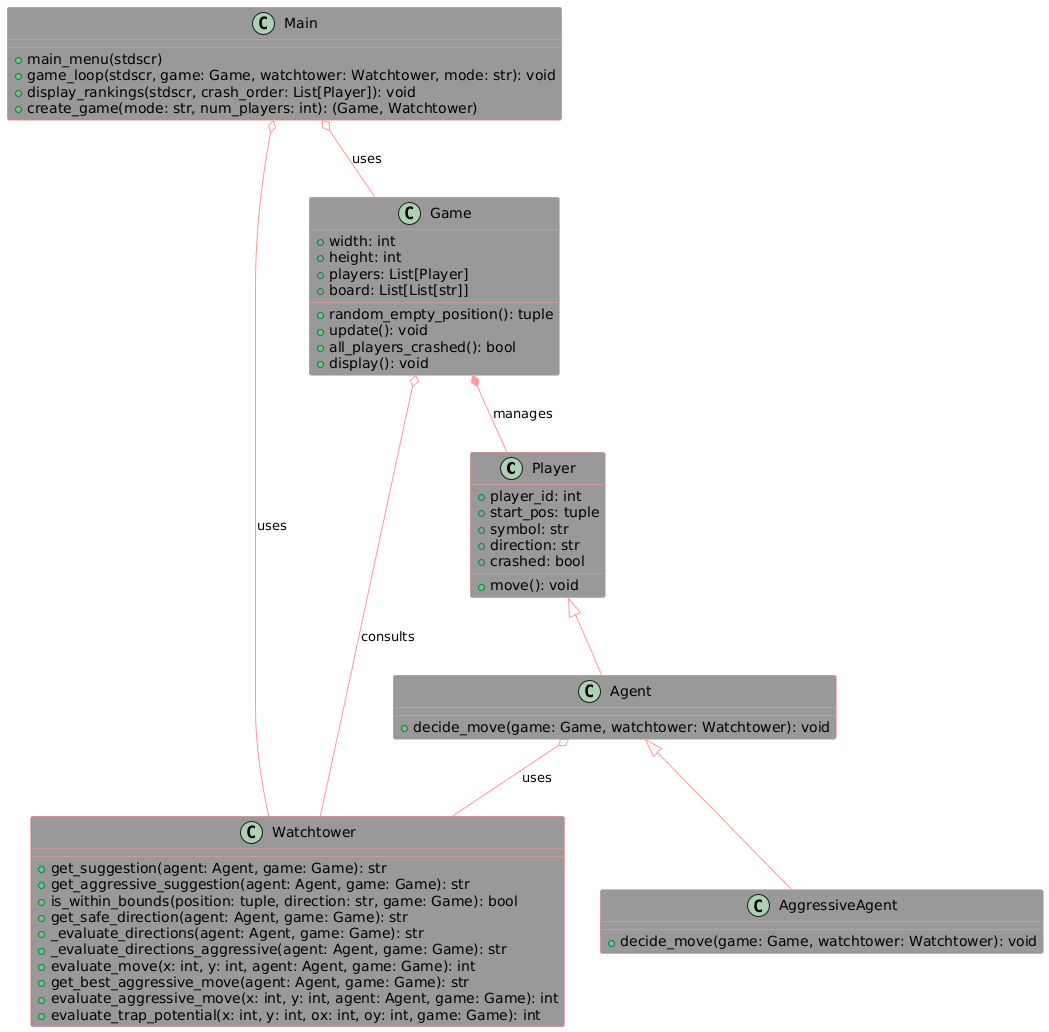
\includegraphics[width=0.8\linewidth]{media/diagram.png}
    \caption{Diagram klas programu}
    \label{fig:enter-label}
\end{figure}


\textbf{Zasada działania programu}\\
Działanie systemu można opisać jako symulację gry wieloosobowej na siatce dwuwymiarowej. System dzieli się na trzy główne fazy:

    \begin{itemize}
        \item Inicjalizacja gry:
        Plansza i gracze są tworzeni na podstawie parametrów określonych w głównym menu.
        Pozycje początkowe graczy są losowane tak, aby nie kolidowały z innymi elementami planszy.

        \item Rozgrywka:
W każdej turze gracze (zarówno użytkownik, jak i agenci) podejmują decyzje dotyczące swoich ruchów: Użytkownik steruje swoim graczem za pomocą klawiszy kierunkowych (W, A, S, D).
Agenci otrzymują sugestie ruchów z \verb|Watchtower| i decydują, czy je zastosować.
Po dokonaniu ruchów stan planszy jest aktualizowany, a gracze, którzy kolidują z przeszkodami lub innymi graczami, są oznaczani jako "rozbici".

        \item Zakończenie gry:
Gra kończy się, gdy wszyscy gracze są rozbici lub na planszy pozostaje tylko jeden aktywny gracz.
Na koniec prezentowana jest tabela wyników z kolejnością graczy, w jakiej odpadli z gry.
    \end{itemize}
\bigskip

\textbf{Funkcje programu}\\
Główne komponenty

    Inicjalizacja planszy:
        Kod odpowiada za stworzenie planszy (board) o zadanych wymiarach oraz inicjalizację pozycji graczy (\verb|random_empty_position| w \verb|Game|).

    Pseudokod:
\begin{lstlisting}
FOR each player IN game.players:
    WHILE True:
        random_position = generate_random_position()
        IF position_empty(random_position):
            player.position = random_position
            break
	\end{lstlisting}

Decyzja o ruchu gracza:

    Gracze sterowani przez komputer (agenci) korzystają z funkcji \verb|decide_move| w \verb|Agent| lub \verb|AggressiveAgent|.
    Ruchy są sugerowane przez \verb|Watchtower| na podstawie:
        Otaczających pól (\verb|evaluate_move|).
        Bliskości przeciwników (\verb|evaluate_aggressive_move|).

Odwołania do równania:

    Funkcja oceniająca pole (\verb|evaluate\_move|) przypisuje punkty na podstawie:
    score=$\sum$(wolne pola - kary za bliskość przeciwników)
    score=$\sum$(wolne pola - kary za bliskość przeciwników)
    W wersji agresywnej nagradzana jest także bliskość przeciwników oraz możliwość ich blokowania: aggressive\_score = odległość do przeciwników + potencjał zablokowania przeciwnika

Aktualizacja stanu gry:

    Plansza jest aktualizowana w każdej turze. Gracze przesuwają się na nowe pozycje, a status kolizji jest weryfikowany.

Pseudokod:
\begin{lstlisting}
    FOR each player IN players:
        player.move()
        IF player.position OUTSIDE bounds OR COLLIDES with another player:
            player.crashed = True
	\end{lstlisting}

    Wyświetlanie wyników:
        Po zakończeniu gry wyświetlana jest tabela z wynikami.

Dzięki modularnej budowie systemu każda część kodu może być rozwijana lub modyfikowana niezależnie. Przykładowo, można łatwo dodać nowe typy agentów lub zmodyfikować logikę ruchów w Watchtower.
    
\newpage
	\subsection*{Testy}
Przeprowadzono trzy rodzaje testów:
\begin{itemize}
    \item testy jednostkowe,
    \item testy funkcjonalne,
    \item testy mutacyjne.
\end{itemize}
Poniżej przedstawiono szczegółowe wyniki i interpretacje każdego z tych rodzajów testów.

\begin{enumerate}
    \item Testy jednostkowe:
    
        Testowane klasy:
        \begin{itemize}
            \item Player ---
                podczas testów tworzony jest obiekt Player oraz sprawdzane jest, czy jego atrybutu zostały poprawnie zainicjalizowane. Następnie sprawdzane jest, czy obiekt poprawnie zmienia swoją pozycję w zależności od kierunku ruchu. 
            \item Agent --- podczas testów tworzone są obiekty Game, Watchtower oraz Agent. Pierwszy test sprawdza, czy agent poprawnie przyjmuje sugestię wieży i zmienia kierunek na ,,Up''. Drugi test sprawdza, czy agent wybiera losowy kierunek z możliwych opcji.
            \item AggressiveAgent --- inicjalizowane są obiekty Game, Watchtower oraz AggressiveAgent. Test sprawdza, czy agent przyjmuje agresywną sugestię wieży i zmienia kierunek na ,,DOWN''.
            \item Watchtower --- inicjalizowane są obiekty Game, Agent oraz Watchtower. Pierwszy test sprawdza, czy wieża zwraca bezpieczny kierunek ,,UP'', gdy pozycja na którą zmierza jest wolna. Drugi test sprawdza, czy wynik oceny ruchu jest typu $int$.
            \item Game --- inicjalizowany jest obiekt Game. Pierwszy test sprawdza poprawność inicjalizacji planszy gry. Drugi test sprawdza, czy metoda $random_empty_position$ zwraca losową pustą pozycję na planszy. Trzeci test sprawdza, czy po wykonaniu ruchu gracza, jego pozycja oraz pozycja na planszy są poprawnie aktualizowane. Ostatni test sprawdza, czy metoda $all_players_crashed$ poprawnie wykrywa, gdy wszyscy gracze ulegli zderzeniu.
        \end{itemize}

        \begin{figure}[H]
            \centering
            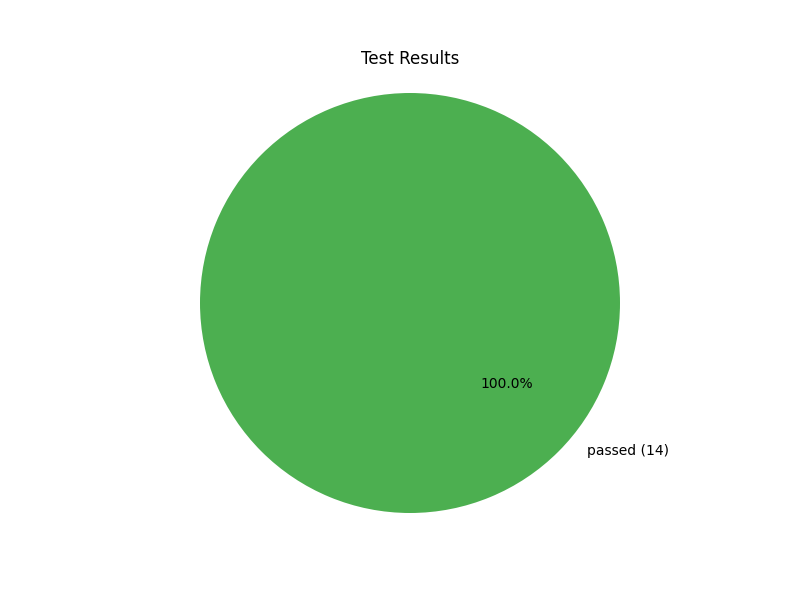
\includegraphics[width=0.8\linewidth]{media/wykresy/unittest.png}
            \caption{Wykres kołowy statusu testów jednostkowych}
            \label{fig:enter-label}
        \end{figure}

    \item Testy funkcjonalne:
        \begin{itemize}
            \item Inicjalizacja gry --- sprawdzanie, czy gra poprawnie uruchamia planszę i jej stan początkowy (wszystkie komórki są puste).
            \item Inicjalizacja gracza --- sprawdza proces umieszczania graczy na planszy. Upewnia się, czy gracze są rozmieszczeni na różnych pozycjach.
            \item Ruch gracza --- sprawdza podstawowe mechanizmy ruchu gracza.
            \item Podejmowanie decyzji przez agenta --- sprawdza proces podejmowania decyzji przez agenta, upewniając się, że każdy agent podejmuje decyzję o kierunku ruchu i że kierunek jest prawidłowy.
            \item Kolizja --- test sprawdza zachowanie na granicach planszy, upewniając się, że gracz oznaczony jest jako $crashed$ po próbie ruchu poza granice planszy.
            \item Logowanie --- test sprawdza funkcjonalność logowania: usuwa istniejący plik logu, tworzy nowy oraz zapisuje zdarzenia i sprawdza, czy plik logu został utworzony i zawiera odpowiednie zdarzenie.
            \item Sugestia wieży --- sprawdza, czy mechanizm sugerowania ruchów przez wieżę działa poprawnie i zawsze zwraca jeden z czterech możliwych kierunków.
            \item Strategia agresywnego agenta --- sprawdza, czy agresywny agent podejmuje decyzje zgodnie z agresywną strategią sugerowaną przez wieżę. 
        \end{itemize}

        \begin{figure}[H]
            \centering
                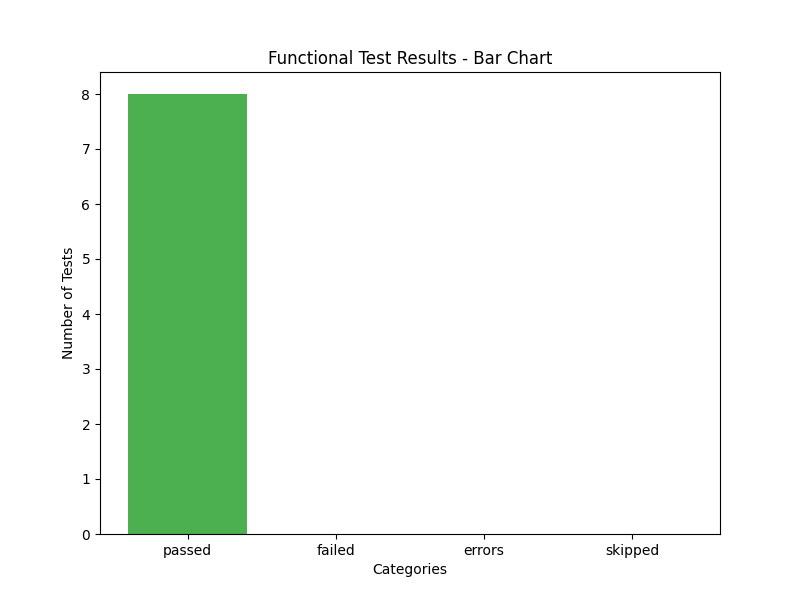
\includegraphics[width=0.8\linewidth]{media/wykresy/bar_functional_test.png}
            \caption{Wykres słupkowy statusu testów funkcjonalnych}
            \label{fig:enter-label}
        \end{figure}

        \begin{figure}[H]
            \centering
                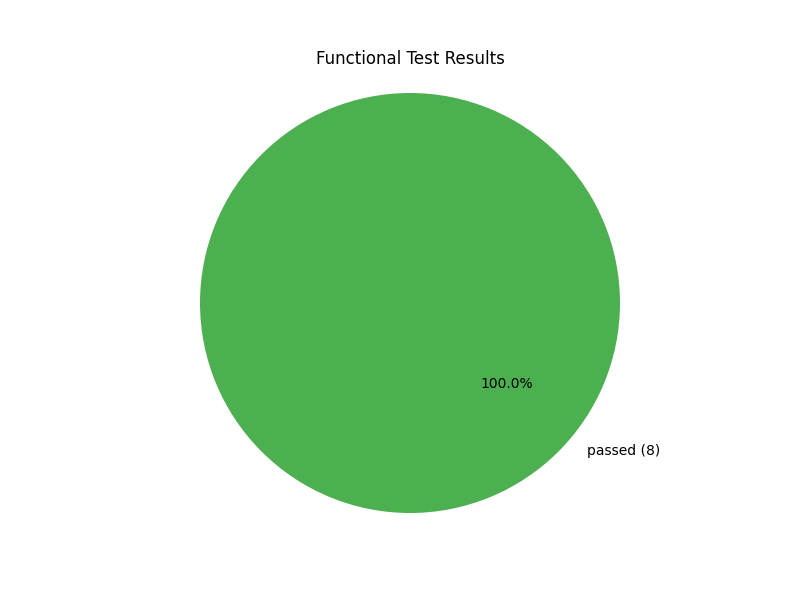
\includegraphics[width=0.8\linewidth]{media/wykresy/pie_functional_test.png}
            \caption{Wykres kołowy statusu testów funkcjonalnych}
            \label{fig:enter-label}
        \end{figure}

    \item Testy mutacyjne:
        Testy mutacyjne dały następujące wyniki:
            \begin{itemize}
                \item Test mutacyjny ukierunkowany na klasę Agent:
                    \begin{figure}[H]
                        \centering
                        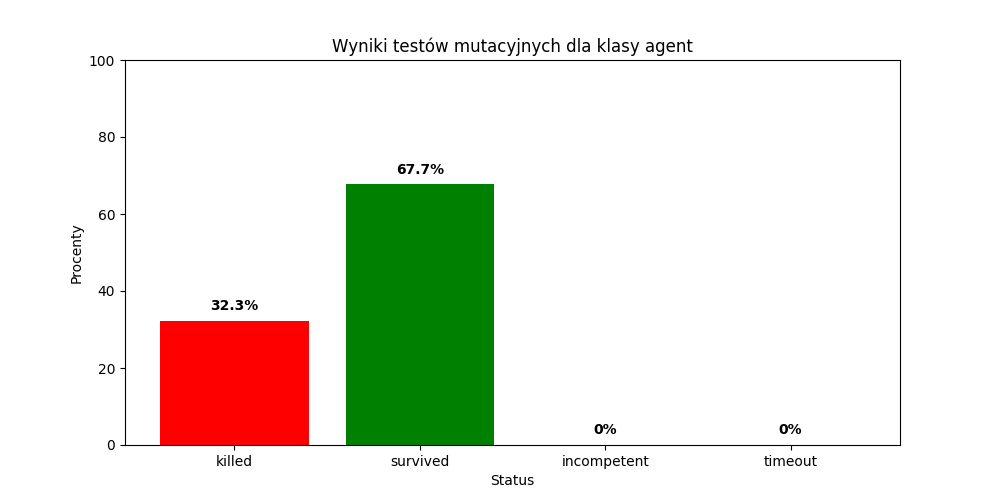
\includegraphics[width=0.8\linewidth]{media/wykresy/bar_agent_mutual_test.png}
                        \caption{Wyniki testów mutacyjnych dla klasy Agent}
                        \label{fig:enter-label}
                    \end{figure}
                    \begin{figure}[H]
                        \centering
                        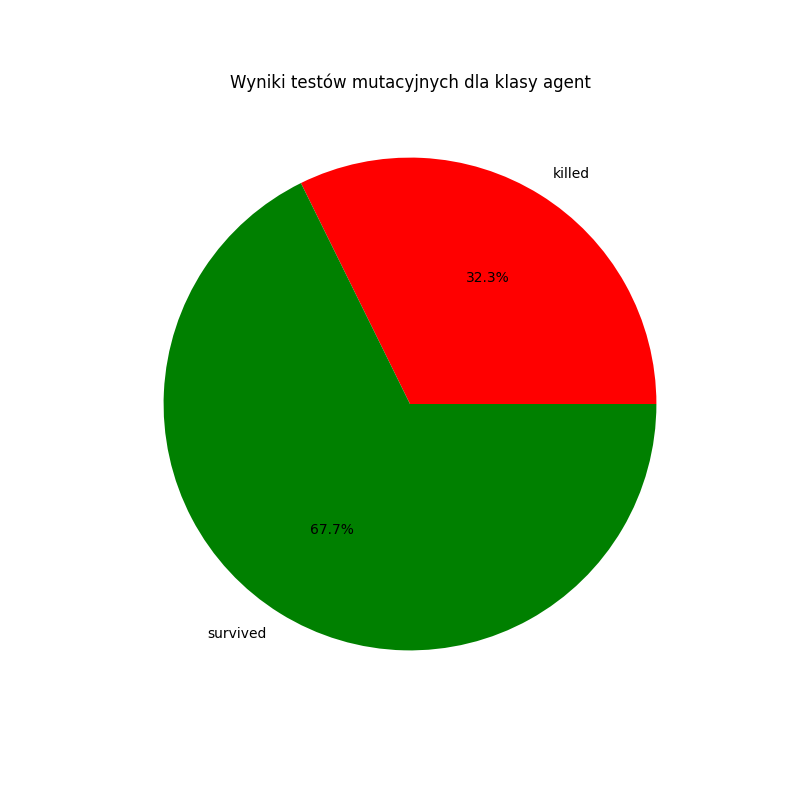
\includegraphics[width=0.8\linewidth]{media/wykresy/pie_agent_mutual_test.png}
                        \caption{Wyniki testów mutacyjnych dla klasy Agent}
                        \label{fig:enter-label}
                    \end{figure}

                    
                \item Test mutacyjny ukierunkowany na klasę Watchtower:
                    \begin{figure}[H]
                        \centering
                        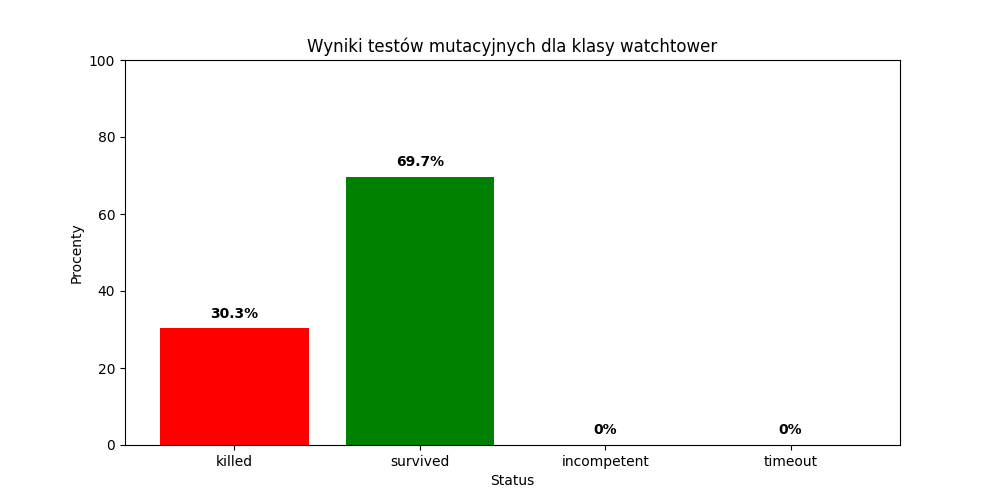
\includegraphics[width=0.8\linewidth]{media/wykresy/bar_watchtower_mutual_test.png}
                        \caption{Wyniki testów mutacyjnych dla klasy Watchtower}
                        \label{fig:enter-label}
                    \end{figure}
                    \begin{figure}[H]
                        \centering
                        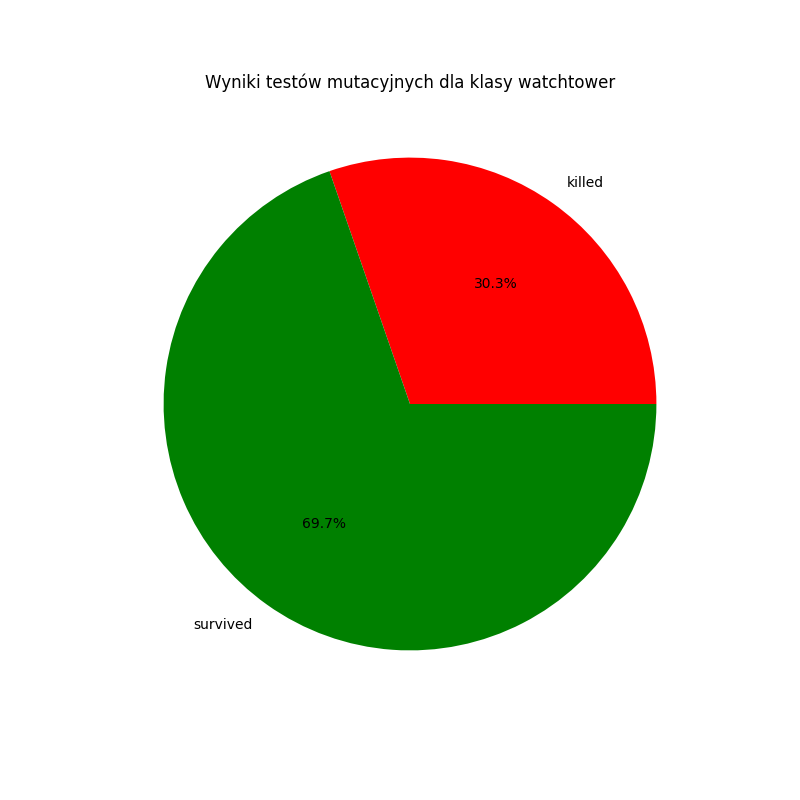
\includegraphics[width=0.8\linewidth]{media/wykresy/pie_watchtower_mutual_test.png}
                        \caption{Wyniki testów mutacyjnych dla klasy Watchtower}
                        \label{fig:enter-label}
                    \end{figure}

                    
                \item Test mutacyjny ukierunkowany na klasę Game:
                    \begin{figure}[H]
                        \centering
                        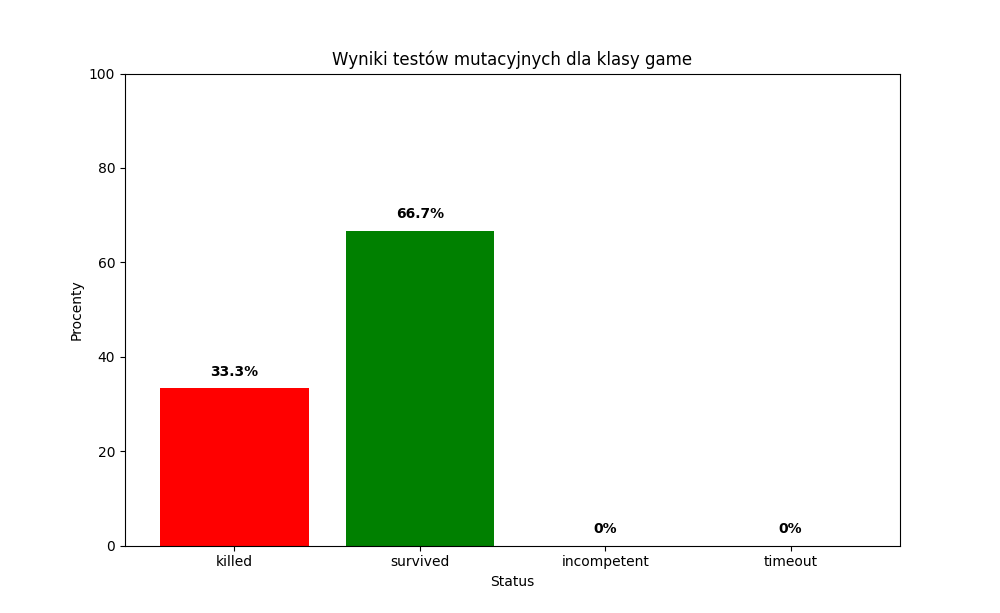
\includegraphics[width=0.8\linewidth]{media/wykresy/bar_game_mutual_test.png}
                        \caption{Wyniki testów mutacyjnych dla klasy Game}
                        \label{fig:enter-label}
                    \end{figure}
                    \begin{figure}[H]
                        \centering
                        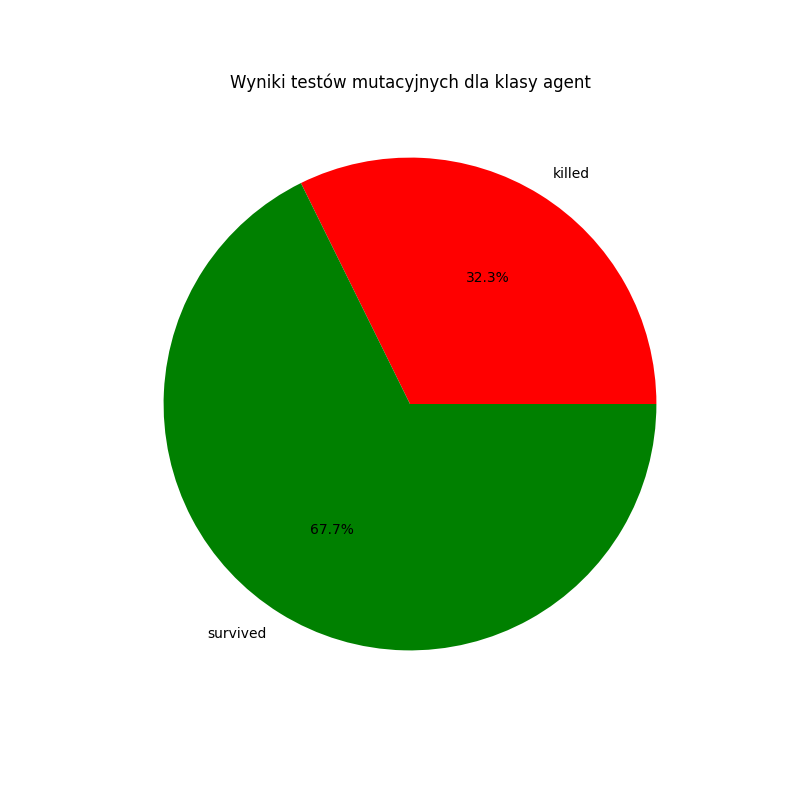
\includegraphics[width=0.8\linewidth]{media/wykresy/pie_agent_mutual_test.png}
                        \caption{Wyniki testów mutacyjnych dla klasy Game}
                        \label{fig:enter-label}
                    \end{figure}
            \end{itemize}

        Słabe wyniki testów mutacyjnych mogą wskazywać na:
        \begin{itemize}
            \item Niewystarczającą liczbę testów jednostkowych.
            \item Niską jakość testów jednostkowych.
            \item Słabe pokrycie kodu.
            \item Niewystarczającą różnorodność testów.
        \end{itemize}

\end{enumerate}


\subsection*{Złożoność oprogramowania} 
Przeprowadźmy kompletną, szczegółową analizę metodą Punktów Funkcyjnych (FPA) dla dostarczonego programu, uwzględniając wagi dla złożoności funkcji.

I. Identyfikacja i Klasyfikacja Funkcji:

Zaczynamy od zidentyfikowania External Inputs (EI), External Outputs (EO) i Logical Internal Files (LIF) oraz przypisania im odpowiedniej złożoności (prosta, średnia, złożona).

1. Zewnętrzne Wejścia (EI):
\begin{itemize}
    \item Wybór trybu gry w menu głównym: Proste (jeden wybór z kilku opcji). Waga: 3
    \item Sterowanie gracza w grze (tryb gracz vs. komputer): Średnie (zmiana kierunku ruchu, wpływ na stan gry). Waga: 4 (Opcjonalne, występuje tylko w trybie gracz vs. komputer).
\end{itemize} 

2. Zewnętrzne Wyjścia (EO):
\begin{itemize}
    \item Wyświetlanie menu gry: Proste (statyczny tekst, kilka opcji). Waga: 4
    \item Wyświetlanie planszy gry: Średnie (dynamiczna aktualizacja, reprezentacja stanu gry, pozycja graczy). Waga: 5
    \item  Wyświetlanie rankingu końcowego: Proste (formatowany tekst z wynikami). Waga: 4
    \item Logowanie do pliku `game\textunderscore logs.txt`: Proste (zapisywanie tekstu, informacje o zdarzeniach i decyzjach agentów). Waga: 4
\end{itemize} 

3. Logiczne Wewnętrzne Typy Plików (LIF):
\begin{itemize}
    \item Reprezentacja planszy gry (`game.board`): Złożona (dwuwymiarowa tablica, przechowywanie stanu każdego pola, detekcja kolizji). Waga: 15
    \item Dane graczy (obiekty klasy `Player`, `Agent`, `AggressiveAgent`): Średnie (przechowywanie pozycji, kierunku, symbolu, stanu `crashed`). Waga: 10
\end{itemize} 

II. Obliczenie Unadjusted Function Points (UFP):

Teraz obliczamy UFP, sumując ważone wartości dla EI, EO i LIF.

Tryb "gracz vs. komputer" (EI = 3 + 4 = 7):
UFP = (7  1) + (17  1) + (25  1) = 7 + 17 + 25 = 49

Tryb "tylko agenci" (EI = 3):
UFP = (3  1) + (17  1) + (25  1) = 3 + 17 + 25 = 45

III. Określenie Wpływu Czynników Projektowych (TDI):

Przypisujemy wagi od 0 do 5 dla każdego z 14 czynników, oceniając ich wpływ na projekt. Poniższe wartości są przykładem i powinny być dostosowane do konkretnego kontekstu.
\begin{itemize}
    \item Komunikacja (między komponentami programu): 3 (istotna, ale nie krytyczna)
    \item Rozproszone przetwarzanie danych: 2 (brak rozproszonego przetwarzania w ścisłym tego słowa znaczeniu)
    \item Wydajność (czas reakcji, płynność gry): 5 (krytyczna dla interaktywnej gry)
    \item Obciążenie (liczba graczy, intensywność aktualizacji): 4 (potencjalnie wysokie obciążenie w grze wieloosobowej)
    \item Częstość transakcji (aktualizacje stanu gry): 3 (umiarkowana, aktualizacje co pewien czas)
    \item Wprowadzanie danych online (interakcja z użytkownikiem): 2 (proste interakcje, wybór menu, sterowanie)
    \item Efektywność (wykorzystanie zasobów): 4 (ważna, szczególnie w kontekście potencjalnego działania w przeglądarce)
    \item Aktualizacja online (aktualizacje oprogramowania): 1 (brak wymogu aktualizacji online w trakcie gry)
    \item Złożoność przetwarzania (algorytmy AI, detekcja kolizji): 3 (umiarkowana złożoność algorytmów)
    \item Wielokrotne wykorzystanie (komponentów kodu): 1 (ograniczony potencjał ponownego użycia)
    \item Łatwość instalacji: 2 (stosunkowo prosta instalacja, uruchomienie skryptu)
    \item Łatwość utrzymania (czytelność kodu, dokumentacja): 3 (kod w miarę modularny, ale wymaga dokumentacji)
    \item Wielostanowiskowość (obsługa wielu graczy): 4 (istotny czynnik, gra wieloosobowa)
    \item Łatwość konfiguracji (parametry gry): 2 (ograniczone opcje konfiguracji)
\end{itemize} 



Obliczenie TDI (Total Degree of Influence):

TDI = 3 + 2 + 5 + 4 + 3 + 2 + 4 + 1 + 3 + 1 + 2 + 3 + 4 + 2 = 39

IV. Obliczenie Adjusted Function Points (AFP):

AFP = UFP  (0.01  TDI + 0.65)

   Dla UFP = 49 (tryb z graczem):
    AFP = 49  (0.01  39 + 0.65)
    AFP = 49  (0.39 + 0.65)
    AFP = 49  1.04
    AFP = 50.96 $\approx$ 51

   Dla UFP = 45 (tryb tylko agenci):
    AFP = 45  (0.01  39 + 0.65)
    AFP = 45  (0.39 + 0.65)
    AFP = 45  1.04
    AFP = 46.8 $\approx$ 47

Podsumowanie:

Ostateczne oszacowanie punktów funkcyjnych (AFP) wynosi około 51 dla trybu z graczem i około 47 dla trybu tylko agenci. Dokładna analiza z uwzględnieniem wag dla złożoności funkcji pozwoliła na uzyskanie bardziej precyzyjnego wyniku. Widać, że czynniki projektowe mają istotny wpływ na ostateczną wartość AFP. Pamiętaj, że kluczowe jest dokładne zrozumienie wymagań i specyfiki projektu przy szacowaniu złożoności funkcji i wpływu czynników projektowych.

	

\end{document}
